\documentclass[11pt]{article}
\usepackage[margin=1in]{geometry}
\usepackage{graphicx,booktabs,hyperref,amsmath}
\graphicspath{{../figures/}}
\title{Characterising the CPU Cache Hierarchy with Microbenchmarks}
\author{Memory System Architecture --- Lab 1}
\date{}
\begin{document}
\maketitle

\section{Overview}
Small, targeted microbenchmarks (\texttt{src/cache\_microbenchmark.cpp}) measure
cache capacity and latency per level, cache line size, and associativity.
Each kernel uses a controlled access pattern and direct timing to isolate one
cache property, and writes its measurements to a CSV file (\texttt{data/}).
All experiments ran on an Intel Xeon Gold 5117 CPU @ 2.00\,GHz.

\section{Pointer-Chasing Latency Kernel}
\paragraph{\texttt{build\_chain}.} Builds a circular linked list inside a buffer.
The buffer is divided into slots separated by a fixed stride; each slot stores a
32-bit index of the next slot.
\begin{itemize}
  \item \textbf{Stride-based layout:} slot $i$ lives at \texttt{buf + i}$\times$\texttt{stride}.
  \item \textbf{Random order:} slot order is shuffled to defeat hardware prefetchers.
  \item \textbf{Circular list:} the last slot points to the first, so traversal needs no bounds checks.
  \item \textbf{Pre-faulted pages:} \texttt{memset} touches every page so no page faults or
        first-touch page walks occur during timing.
\end{itemize}

\paragraph{\texttt{measure\_access\_time}.}
\begin{enumerate}
  \item Allocate a 64-byte aligned buffer with \texttt{posix\_memalign}.
  \item Build a randomised pointer chain over the buffer.
  \item Traverse the chain once to warm the caches.
  \item Traverse it again, timed with \texttt{clock\_gettime(CLOCK\_MONOTONIC)}.
  \item Divide elapsed time by the number of accesses.
\end{enumerate}
Each load depends on the previous one, so loads cannot overlap and the measured
time is the latency of whichever level services the access.

\section{Cache Hierarchy: Capacity and Latency}
The pointer-chasing kernel is run for working sets from 1\,KB to several GB,
with the stride fixed at one cache line so every access touches a new line.
When the working set outgrows a level, accesses spill to the next level and
latency steps up.

\begin{figure}[h]
  \centering
  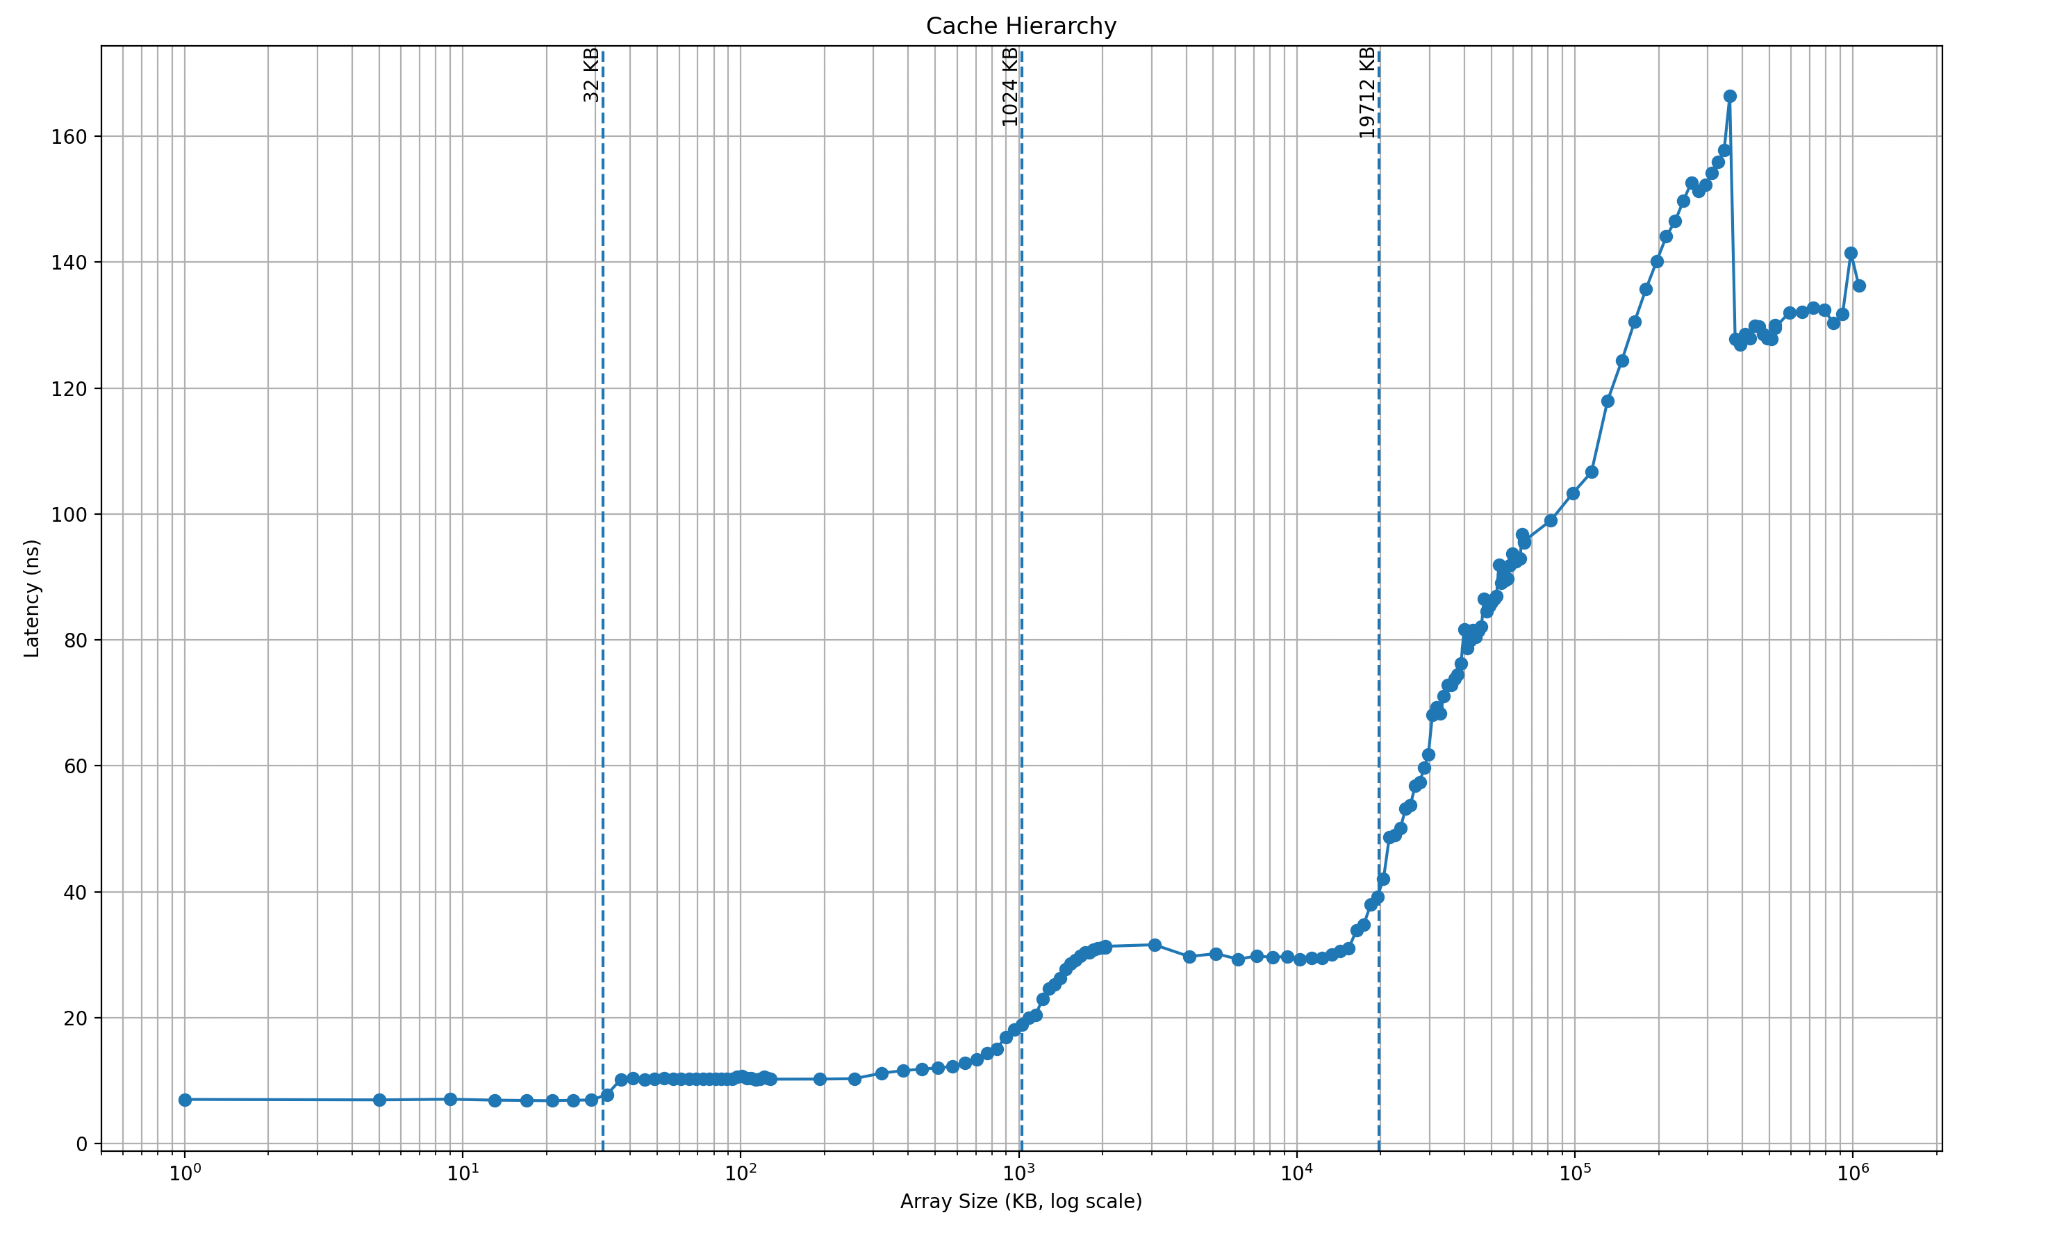
\includegraphics[width=0.85\linewidth]{cache_hierarchy.png}
  \caption{Average dependent-load latency vs.\ working-set size (log scale).
           Dashed lines mark 32\,KB, 1\,MB and 19.25\,MB.}
\end{figure}

\begin{table}[h]
  \centering
  \begin{tabular}{lcc}
    \toprule
    Level & Capacity (knee) & Latency plateau \\
    \midrule
    L1   & $\approx$ 32\,KB & 4--6\,ns \\
    L2   & $\approx$ 1\,MB  & 10--12\,ns \\
    L3   & $\approx$ 20\,MB & 37--39\,ns \\
    DRAM & ---              & $\approx$ 130\,ns \\
    \bottomrule
  \end{tabular}
  \caption{Capacities and latencies read from the hierarchy curve.}
\end{table}

The transient spike to $\approx$160\,ns at intermediate large sizes is caused by
TLB misses and page-walk overhead; it subsides once large-page backing reduces
translation cost.

\section{Cache Line Size}
\paragraph{\texttt{measure\_cache\_line\_size}.} For increasing offsets $\Delta$:
\begin{enumerate}
  \item Pick addresses $p_0$ and $p_1 = p_0 + \Delta$.
  \item Evict both from every level with \texttt{clflush}, then \texttt{\_mm\_mfence()}.
  \item Load $p_0$, bringing exactly one line into the cache.
  \item Time the access to $p_1$ with \texttt{rdtscp}, fenced by \texttt{\_mm\_lfence()}.
\end{enumerate}
If $p_1$ shares $p_0$'s line it hits; once $\Delta$ exceeds the line size it misses.

\begin{figure}[h]
  \centering
  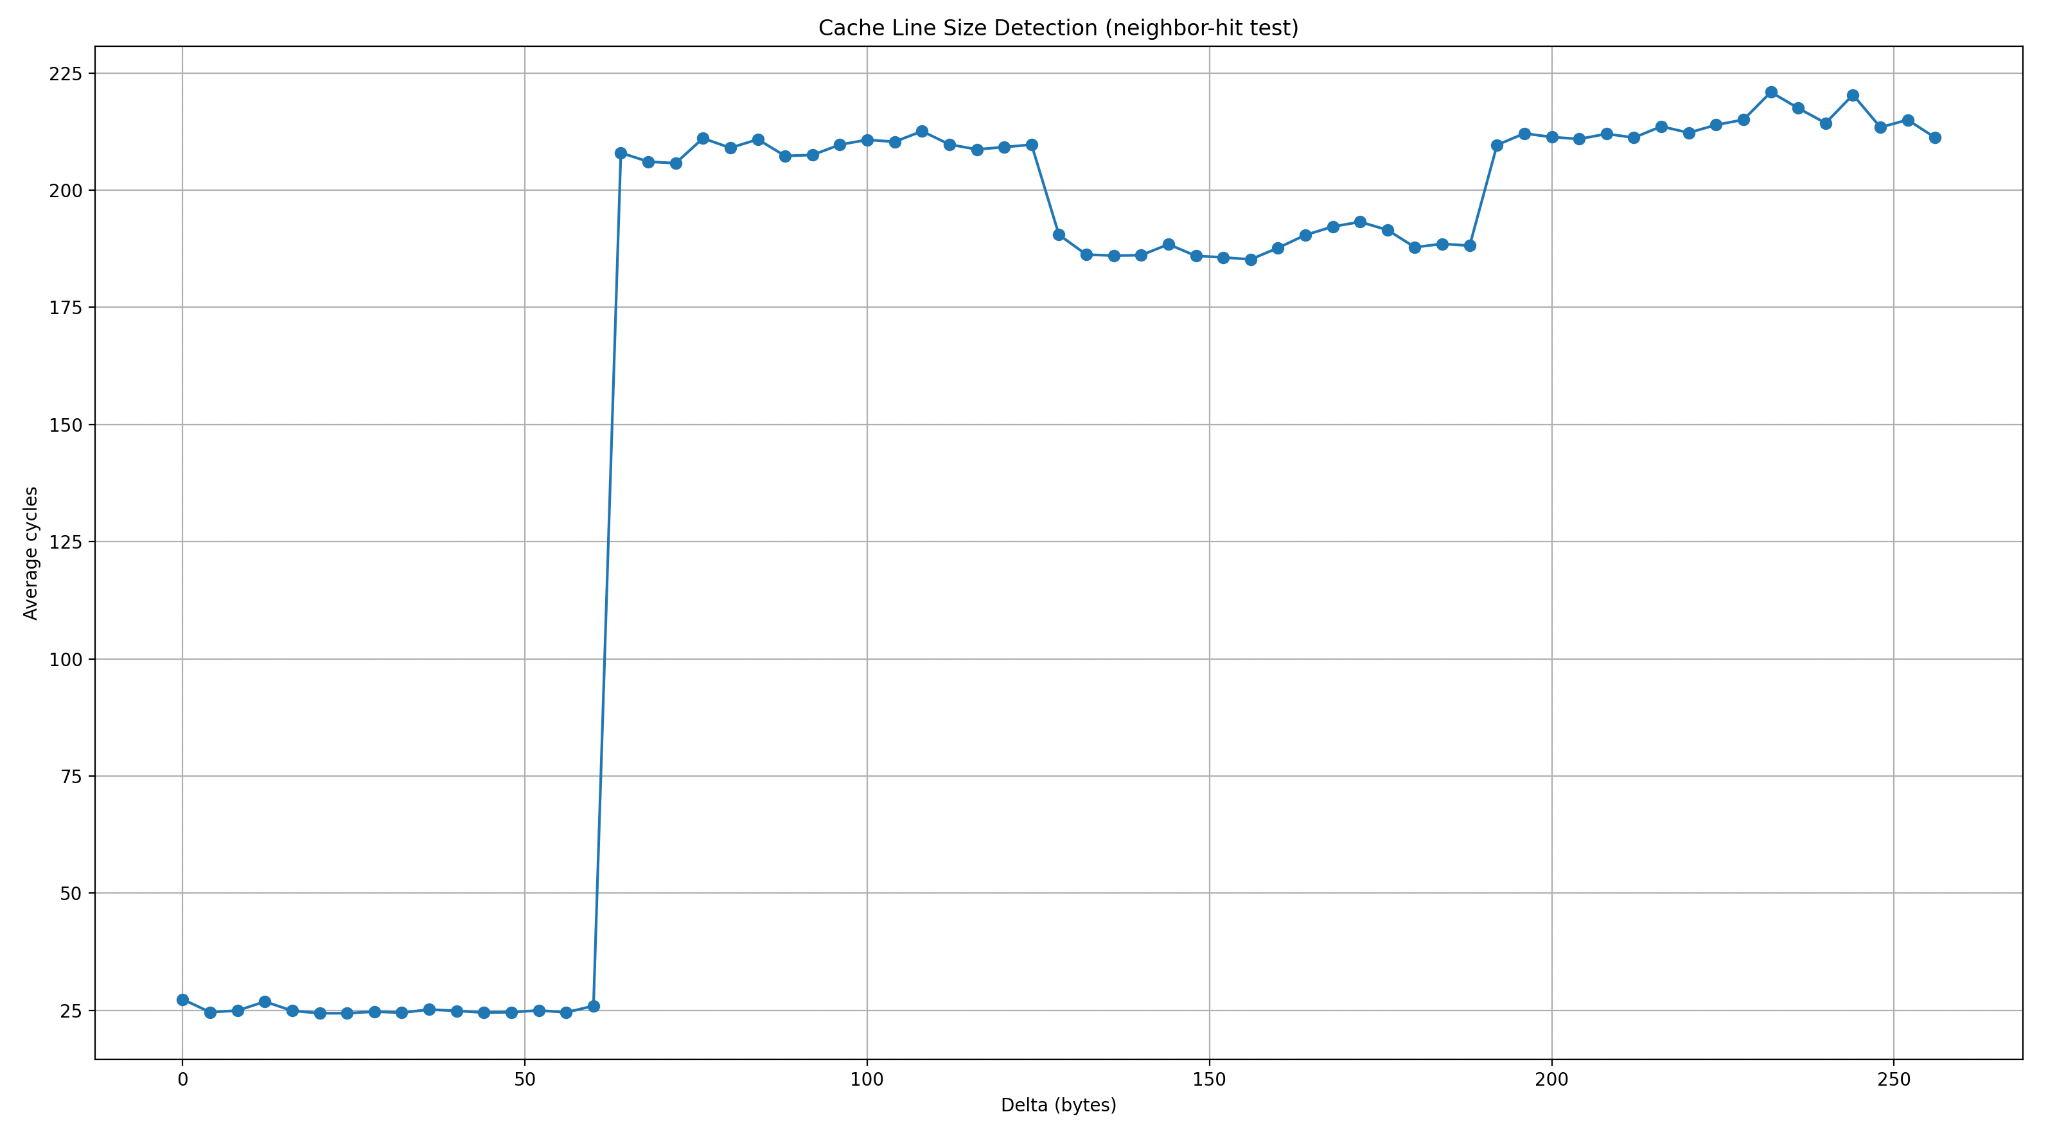
\includegraphics[width=0.8\linewidth]{cache_line_size.png}
  \caption{Access time to $p_1$ vs.\ offset $\Delta$. The knee at 62--64\,B gives a 64-byte line.}
\end{figure}

\section{Associativity}
\paragraph{\texttt{measure\_cache\_associativity}.}
\begin{enumerate}
  \item Allocate a page-aligned (4\,KB) buffer to keep index bits consistent.
  \item Load a 64-byte aligned victim line.
  \item Access $N$ further lines spaced by the cache size, so all map to the victim's set.
  \item Time a reload of the victim with \texttt{rdtscp} and fences.
\end{enumerate}
When $N$ exceeds the associativity the victim is evicted and the reload slows down.
The same procedure is repeated with a spacing of 32\,KB, 1\,MB and 19.25\,MB for L1, L2 and L3.

\begin{figure}[h]
  \centering
  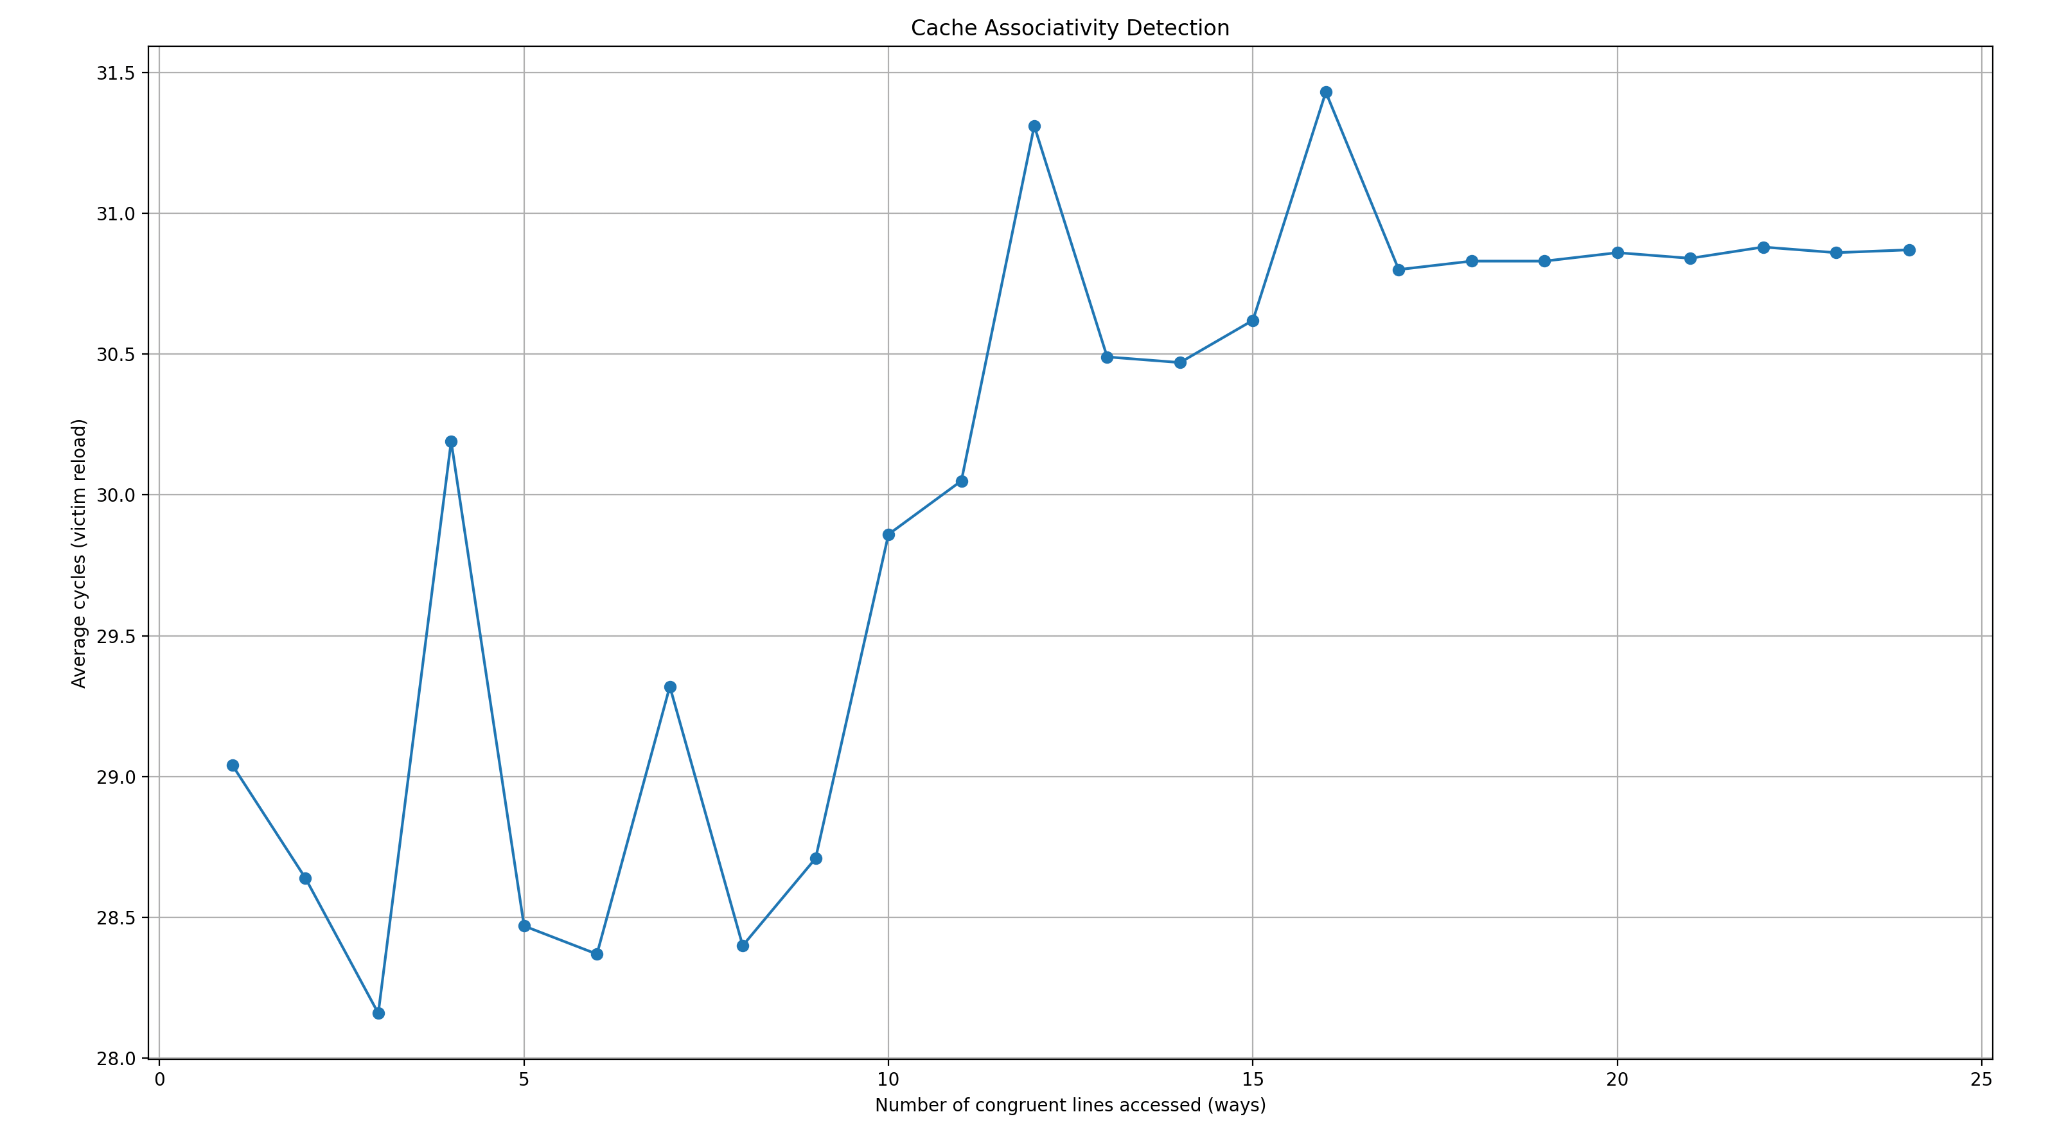
\includegraphics[width=0.32\linewidth]{l1_associativity.png}\hfill
  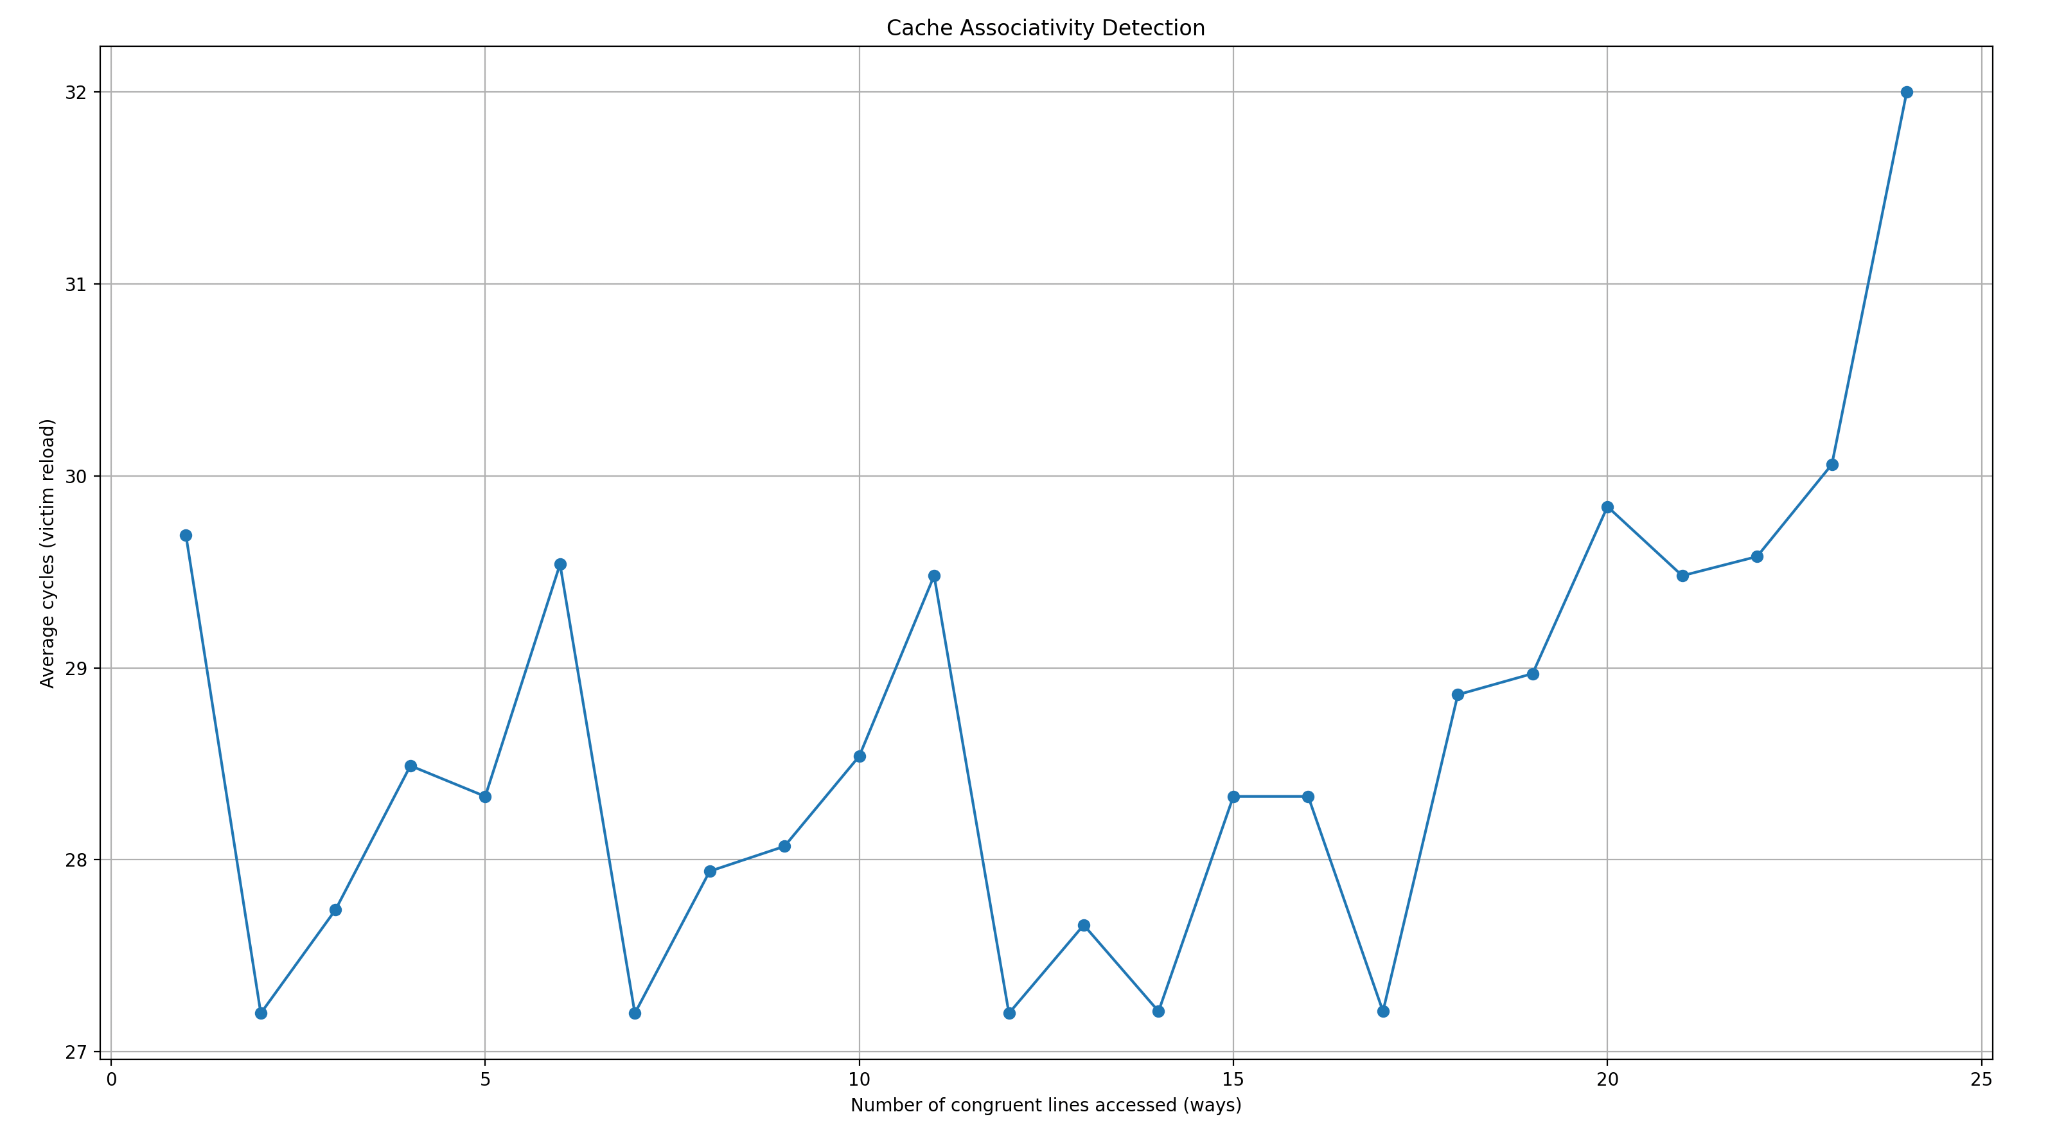
\includegraphics[width=0.32\linewidth]{l2_associativity.png}\hfill
  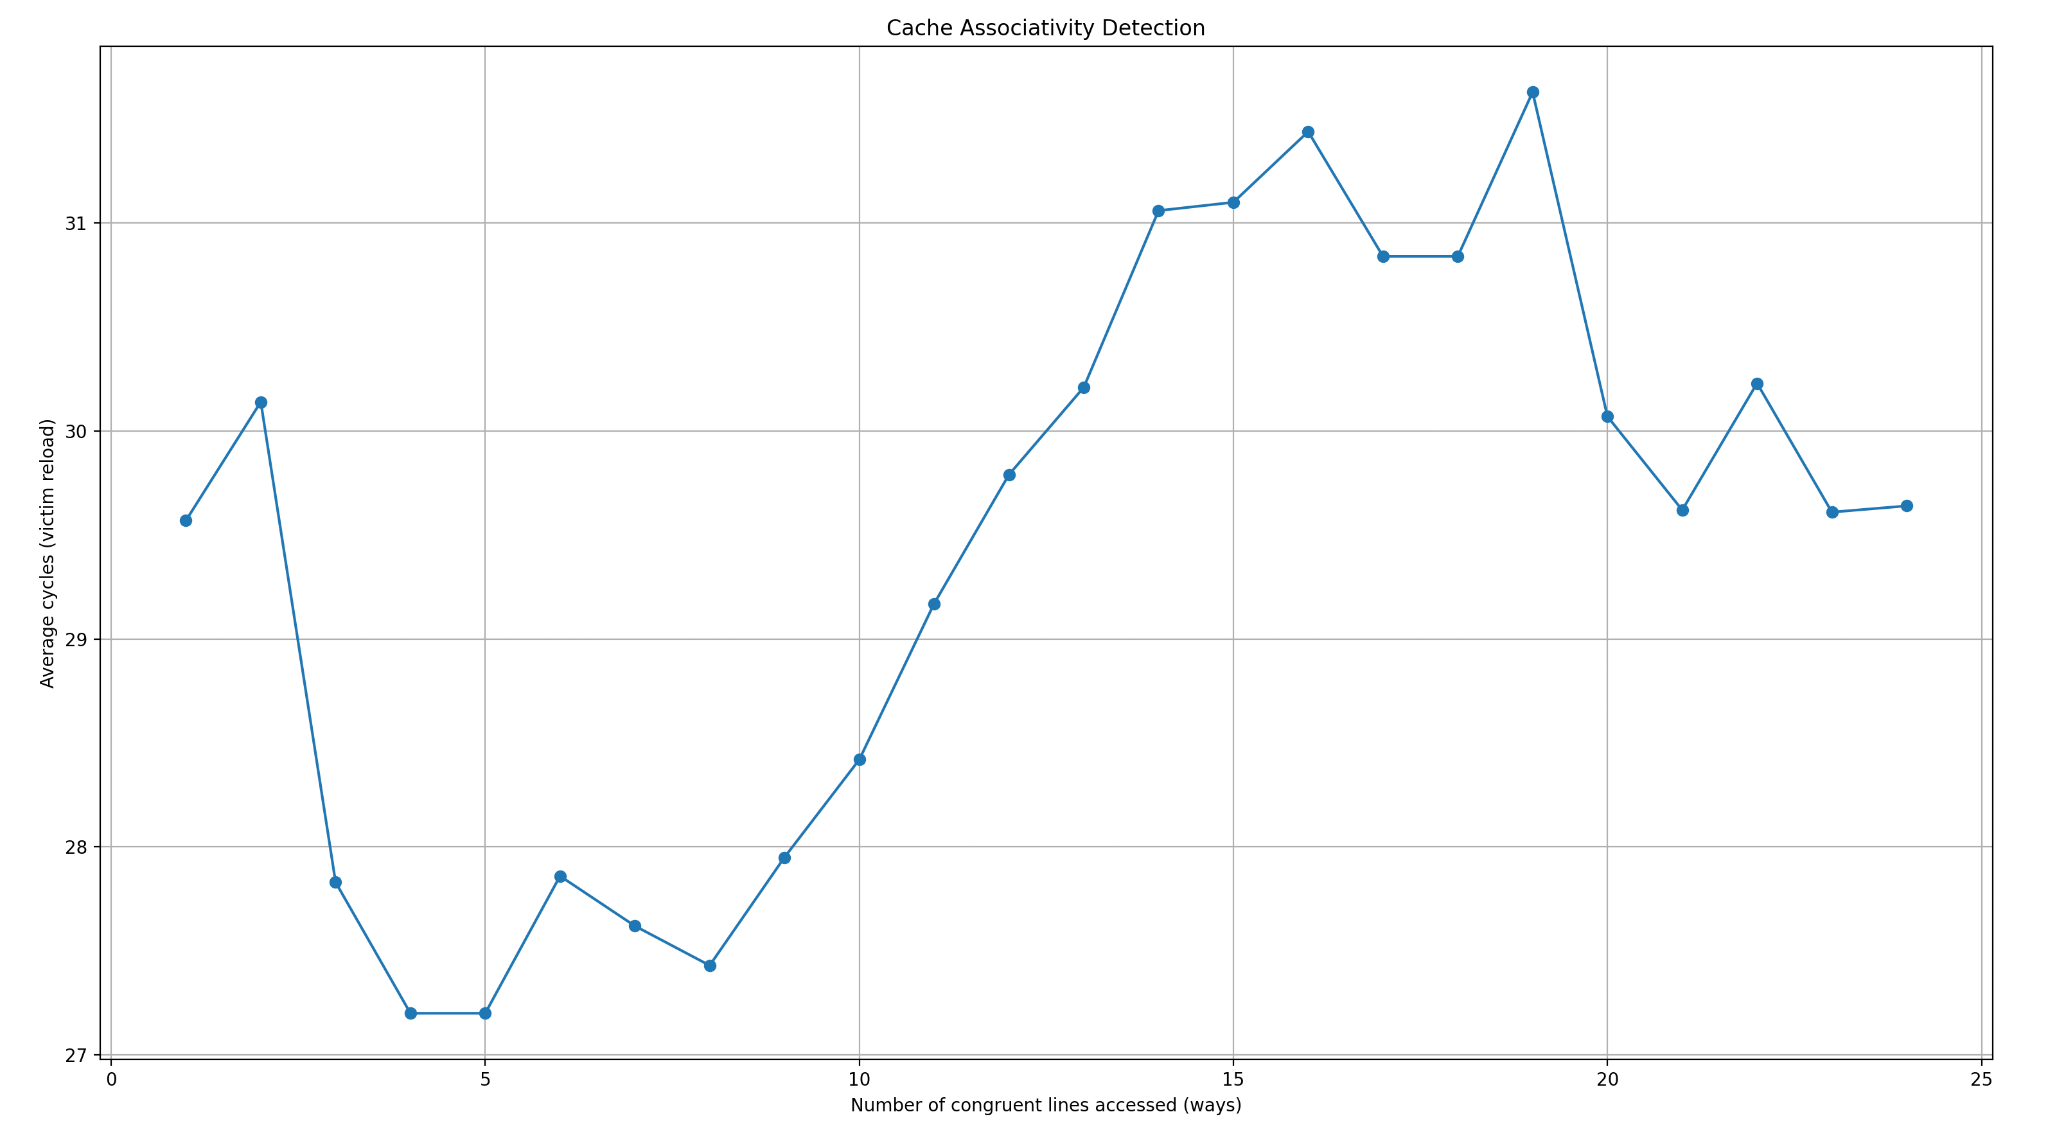
\includegraphics[width=0.32\linewidth]{l3_associativity.png}
  \caption{Victim reload time vs.\ number of congruent lines: L1 (left), L2 (centre), L3 (right).}
\end{figure}

\begin{itemize}
  \item \textbf{L1:} reload stays at $\approx$28--29 cycles up to 8 lines and rises to $\approx$31 beyond:
        \textbf{8-way}. Transitions are soft because replacement is not strict LRU.
  \item \textbf{L2:} transition at \textbf{16 ways}.
  \item \textbf{L3:} apparent transition at 8 ways, below the documented 11 ways. The L3 is
        shared and sliced, and its address hash spreads the lines across slices, so they do not all
        compete for a single set.
\end{itemize}

\section{Results Summary}
\begin{table}[h]
  \centering
  \begin{tabular}{lccc}
    \toprule
    & L1 & L2 & L3 \\
    \midrule
    Capacity      & 32\,KB & 1\,MB & $\approx$20\,MB \\
    Latency       & 4--6\,ns & 10--12\,ns & 37--39\,ns \\
    Associativity & 8 & 16 & 8 (measured, see text) \\
    \midrule
    \multicolumn{4}{l}{Line size: 64\,B \quad DRAM latency: $\approx$130\,ns} \\
    \bottomrule
  \end{tabular}
\end{table}

\section{Conclusion}
Dependent loads, explicit flushes and cycle-accurate timing expose the capacity,
latency, line size and associativity of each cache level, and the results agree with
the Xeon Gold 5117's published specification for L1/L2. Residual noise comes from
non-LRU replacement, hardware prefetching, OS scheduling, frequency scaling and TLB
effects, but every transition point remains clearly visible.

\end{document}
